\documentclass[12pt]{article}
\usepackage{amsfonts}
\usepackage{amsmath}
\usepackage{bm}
\usepackage{bbm}
\usepackage{graphicx}
\usepackage{geometry}[margin=1in]
\usepackage{subcaption}
\usepackage{array}

% for algorithms
\usepackage[linesnumbered,ruled]{algorithm2e}

\usepackage{natbib}
\usepackage{multicol}
\bibliographystyle{plainnat}
% set path for bibliography

\title{Regionally Additive Models: Explainable-by-design models minimizing feature interactions}

\newcommand{\dfdx}{\frac{\partial f}{\partial x_s}}
\newcommand{\Rd}{\mathbb{R}^d}
\newcommand{\xb}{\mathbf{x}}
\newcommand{\xc}{\mathbf{x_c}}
\newcommand{\xcc}{\mathbf{x_{/s}}}
\newcommand{\fxc}{f^{(\xc)}}
\newcommand{\fxs}{f^{(x_s)}}
\newcommand{\Xcal}{\mathcal{X}}
\newcommand{\Ycal}{\mathcal{Y}}
\newcommand{\when}[1]{\mathbbm{1}_{#1}}

\author{Vasilis Gkolemis}


\begin{document}
\maketitle

\begin{abstract}
Generalized Additive Models (GAMs) are a popular class of explainable-by-design models that are widely used in practice.
GAMs are based on the assumption that the effect of each feature on the target is independent of the values of the
other features, however, in cases where this assumption is violated they may lead to poor performance.
To address this limitation we propose Regionally Additive Models (RAMs), a novel class of explainable-by-design models,
that fits multiple GAMs to subregions of the feature space where interactions are minimized.
Our approach consists of two steps: first, we fit a black-box model and we identify the subregions where the black-box model is nearly locally additive,
i.e., where the effect of each feature on the target is independent of the values of the other features.
Secondly, we train a GAM specifically for each identified subregion.

We show that RAMs are more expressive than GAMs while they are still interpretable.

\end{abstract}

\section{Introduction}


% Paragraph for Motivating about Regionally Additive Models
Generalized Additive Models (GAMs)~\citep{hastie1987generalized} are a popular class of explainable by design (x-by-design) models.
Their popularity stems from their seamless interpretability; since they are a linear (additive) combination of univariate functions,
\(f(\xb) = c + \sum_{s=1}^D f_s(x_s)\), each individual univariate function (component) can be readily visualized and comprehended in isolation.
However, GAM's main limitation is that they cannot express interactions between features.
To mitigation this limitation, some approaches~\citep{lou2013accurate} extend them enabling pairwise interactions,
i.e., \(f(\xb) = c + \sum_{s=1}^D f_s(x_s) + \sum_{s=1}^D \sum_{c \neq s} f_{sc}(x_s, x_c)\).
Pairwise interactions can also be visualized and understood in isolation, so these models also maintain their x-by-design nature.
Unfortunately, this does not hold for any interaction that involves more than two features, thus, the expressiveness of GAMs is limited to capturing up to two-feature interactions.

% Paragraph for Motivating about Regionally Additive Models
To overcome this limitation, we propose Regionally Additive Models (RAMs), a novel class of x-by-design models,
that fits multiple GAMs to subregions of the feature space where interactions are minimized.
Our approach consists of a three-step pipeline.
First, we fit a black-box model to capture all high-order interactions.
Second, we identify the subregions where the black-box model is nearly locally additive.
Finally, we train a GAM specifically for each identified subregion.

\section{Background and motivation}
\label{sec:motivation}

Consider the black-box function \(f(\xb) = 8x_2\when{x_1 > 0}\when{x_3=0}\)
with \(x_1, x_2 \sim \mathcal{U}(-1,1)\) and \(x_3 \sim Bernoulli(0,1)\).
Although very simple, a GAM would fail to learn this mapping due to
the existence of the three-features interaction term $8x_2\when{x_1 > 0}\when{x_3=0}$.
As we see in Figure~\ref{subfig:global_gam}, a GAM misleadingly learns that $\hat{f}(\xb) \approx 2x_2$,
because in $\frac{1}{4}$ of the cases ($x_1 > 0 \text{ and } x_3 = 0$) the impact of $x_2$ to the output is $8x_2$,
and in the rest $\frac{3}{4}$ of the cases the impact of $x_2$ to the output is $0$.
However, if splitting the input space in two subregions we observe that \(f\) is additive in each one (regionally additive):
%
\begin{equation}
    \label{eq:regionally_additive}
    f(\xb) = \begin{cases} 8x_2 & \text{if } x_1 > 0 \text{ and } x_3 = 1 \\ 0 & \text{otherwise} \end{cases}
\end{equation}
%
Therefore, if we knew the appropriate subregions,
namely, \(\mathcal{R}_{21} = \{x_1 > 0 \text{ and } x_3 = 0\}\)
and  \(\mathcal{R}_{22} = \{x_1 \leq 0 \text{ or } x_3 = 1\}\),
we could split the impact of $x_2$ appropriately and fit the following model to the data:

\begin{equation}
    \label{eq:regional_gam}
    f^{\mathtt{RAM}}(\xb) = f_1(x_1) + f_{21}(x_2) \when{(x_1, x_3) \in \mathcal{R}_{21}} + f_{22}(x_2) \when{(x_1, x_3) \in \mathcal{R}_{22}} + f_3(x_3)
\end{equation}
%
Equation~\eqref{eq:regional_gam} represents a Regionally Additive Model (RAM), which is simply a GAM fitted on each subregion of the feature space.
Importantly, RAM's enhanced expressiveness does not come at the expense of interpretability.
As we observe in Figures~\ref{subfig:regional_gam_1} and~\ref{subfig:regional_gam_2}, we can still visualize and comprehend each univariate function in isolation, exactly as we would do with a GAM,
with the only difference being that we have to consider the subregions where each univariate function is active,
The key challenge of RAMs is to appropriately identify the subregions where the black-box function is (close to) regionally additive.
For this purpose, as we will see in Section~\ref{subsec:regional_effect_methods}, we propose a novel algorithm that is based on the idea of
regional effect plots.

\begin{figure}[htbp]
    \centering
    \begin{subfigure}{0.32\textwidth}
        \centering
        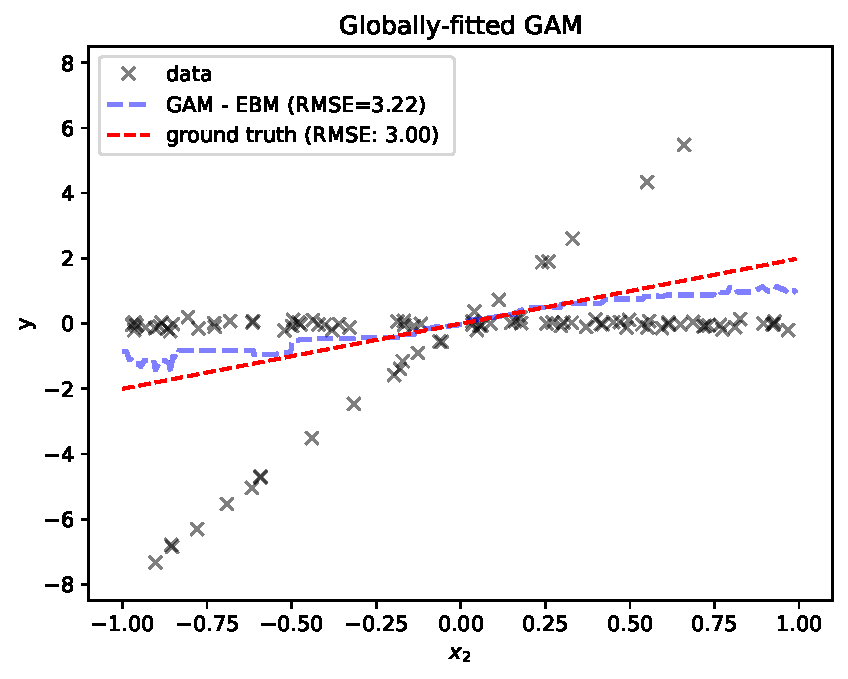
\includegraphics[width=\textwidth]{figures/global_GAM}
        \caption{\(f_2(x_2)\)}
        \label{subfig:global_gam}
    \end{subfigure}
    \begin{subfigure}{0.32\textwidth}
        \centering
        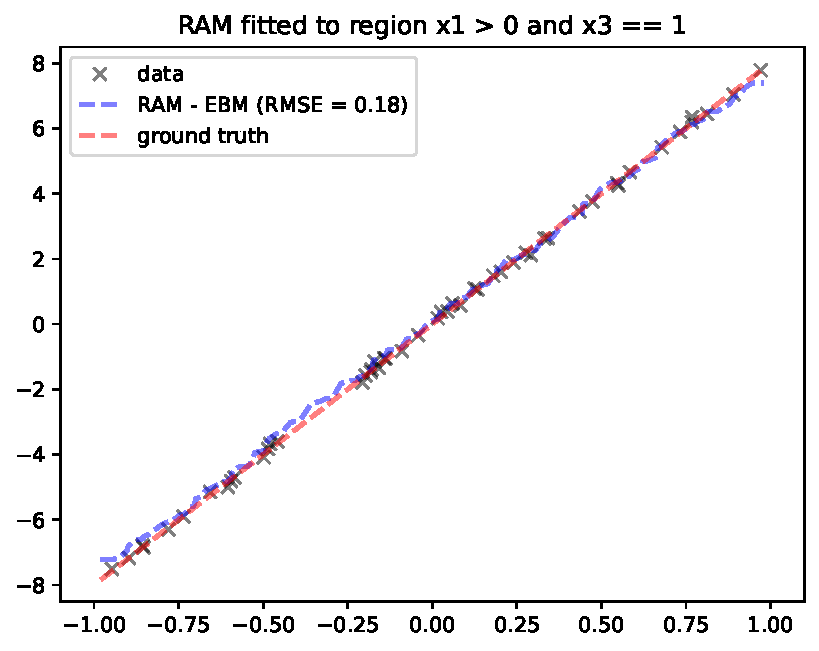
\includegraphics[width=\textwidth]{figures/regional_gam_subreg_1}
        \caption{\(f_2(x_2) \when{x_1 > 0 \text{ and } x_3 = 1}\)}
        \label{subfig:regional_gam_1}
    \end{subfigure}
    \begin{subfigure}{0.32\textwidth}
        \centering
        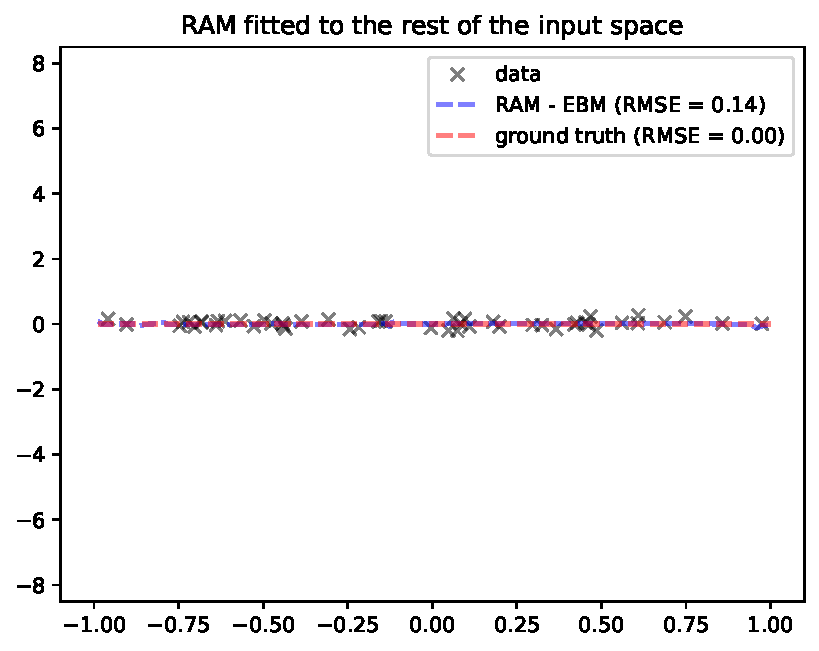
\includegraphics[width=\textwidth]{figures/regional_gam_subreg_2}
        \caption{\(f_2(x_2) \when{x_1 \leq 0 \text{ or } x_3 \neq 1}\)}
        \label{subfig:regional_gam_2}
    \end{subfigure}
    \caption{Caption for the entire figure}
    \label{fig:ram_example}
\end{figure}


\section{The RAM framework}

\subsection{Background}

Let \(\Xcal \in \Rd\) be the \(d\)-dimensional feature space, \(\Ycal\) the target space and \(f(\cdot) : \Xcal \rightarrow \Ycal\) the black-box function.  We use index \(s \in \{1, \ldots, d\}\) for the feature of interest and \(c = \{1, \ldots, d\} - s\) for the rest.
For convenience, we use \((x_s, \xcc)\) to refer to \((x_1, \cdots , x_s, \cdots, x_D)\) and, equivalently, \((X_s, X_c)\) instead of \((X_1, \cdots , X_s, \cdots, X_D)\) when we refer to random variables.
The training set \(\mathcal{D} = \{(\xb^i, y^i)\}_{i=1}^N\) is sampled
i.i.d.\ from the distribution \(\mathbb{P}_{X,Y}\).  Finally,
\(f^{\mathtt{<method>}}(x_s)\) denotes how \(\mathtt{<method>}\)
defines the feature effect and \(\hat{f}^{\mathtt{<method>}}(x_s)\)
how it estimates it from the training set.

\subsection{Fit a black-box function}

\subsubsection{Objective}

In the first step of the pipeline, a black-box function \(f(\cdot)\) is fitted to the training set \(\mathcal{D} = \{(\xb^i, y^i)\}_{i=1}^N\).
In principle, the black-box function can be any model that is expressive enough to accurately fit the data,
meaning that it is able to learn the underlying mapping \(\mathbb{P}_{Y|X}\).

\subsubsection{Proposed Approach}

For being able to use the DALE approximation that we propose in the next step,
the black-box function should be differentiable.
Recent developments have shown that differentiable Deep Learning models specifically designed for tabular
data~\citep{arik2021tabnet} can achieve state-of-the-art performance, make them a good candidate for this step.
In the running example, we use a simple neural network with three hidden layers as the black-box function,
which achieves a test \(\texttt{MSE} \approx 0.01\).
The neural network is trained using the Adam optimizer (add citation) with a learning rate of \(0.01\).
Based on the small test \(\texttt{MSE}\), we can assume that the neural network is able to capture any interactions
between the features.

\subsection{Regions that minimize feature interactions}
\label{subsec:regional_effect_methods}

In this step, we use regional effect methods to identify the regions where the black-box function is nearly locally additive.

\subsubsection{Objective}

% Describe the goal of the regional effect methods
Regional effect methods yield for each individual feature \(s\), a set of \(T_s\) non-overlapping regions,
denoted as \(\{\mathcal{R}_{st}\}_{t=1}^{T_s}\) where \(\mathcal{R}_{st} \subseteq \Xcal_{/s}\).
Note that, first, we use a subscript, i.e. $T_s$, to denote that the number of non-overlapping regions can be different for each feature and, second,
the regions \(\{\mathcal{R}_{st}\}_{t=1}^{T_s}\) are disjoint and their union covers the entire feature space \(\Xcal_{/s}\).
The primary objective is to identify regions in which the impact of the \(s\)-th feature on the output is
\textit{relatively independent} of the values of the other features \(\xcc\).
To better grasp this objective, if we decompose the impact of the \(s\)-th feature on the output $y$ into two terms:
\(f_s(x_s, \xcc) = f_{s,ind}(x_s) + f_{s, int}(x_s, \xcc)\),
where \(f_{s,ind}(\cdot)\) represents the independent effect
and \(f_{s, int}(\cdot)\) represents the interaction effect,
the objective is to identify regions \(\{\mathcal{R}_{st}\}_{t=1}^{T_s}\) such that the interaction effect is minimized.
Regionally Additive Models (RAM) formulation is:

\begin{equation}
\label{eq:ram_formulation}
f^{\mathtt{RAM}}(\xb) = c + \sum_{s=1}^D \sum_{t=1}^{T_s} f_{st}(x_s) \when{\xcc \in \mathcal{R}_{st}}
\end{equation}
%
In the above formulation, \(f_{st}(\cdot)\) is the component of the \(s\)-th feature which is active on the \(t\)-th region.
RAM can be viewed as a GAM with \(T_s\) components per feature where each component is applied to a specific region \(\mathcal{R}_{st}\).
To facilitate this interpretation, we can define an enhanced feature space \(\Xcal^\mathtt{RAM}\) defined as:

\begin{equation}
\label{eq:ram_feature_space}
\begin{aligned}
\Xcal^{\mathtt{RAM}} &= \{x_{st} | s \in \{1, \ldots, D\}, t \in \{1, \ldots, T_s\}\} \\
x_{sk} &= \begin{cases}
x_s, & \text{if } \xcc \in \mathcal{R}_{sk} \\
0, & \text{otherwise}
\end{cases}
\end{aligned}
\end{equation}
%
and then define RAM as a typical GAM on the extended feature space \(\Xcal^{\mathtt{RAM}}\):

\begin{equation}
\label{eq:ram_formulation2}
f^{\mathtt{RAM}}(\xb) = c + \sum_{s,t} f_{st}(x_{st})
\end{equation}
%
In the running example, to minimize the effect of feature interactions, we have to split the effect of feature \(x_2\) into two regions,
\(\mathcal{R}_{21} = \{x_1 > 0 \text{ and } x_3 = 1\}\) and \(\mathcal{R}_{22} = \{x_1 \leq 0 \text{ or } x_3 = 0\}\).
The RAM formulation is \(f^{\mathtt{RAM}}(\xb) = f_1(x_1) + f_{21}(x_{21}) + f_{22}(x_{22}) + f_3(x_3)\).


\subsubsection{Proposed Approach}

To identify the regions of the input space where the impact of feature interactions is reduced,
we have developed a regional effect method influenced by the research conducted by
\citet{herbinger2023decomposing} and \citet{gkolemis2023dale}.
\citet{herbinger2023decomposing} introduced a versatile framework for detecting such regions,
where one of the proposed methods is the Accumulated Local Effects~\citep{apley2020visualizing}.
We have adopted their approach with two notable modifications.
First, instead of using the ALE plot, we employ the Differential ALE (DALE) method introduced by \citet{gkolemis2023dale},
which provides considerable computational advantages when the underlying black-box function is differentiable.
Second, we utilize variable-size bins, instead of the fixed-size ones in DALE, because the result in a more accurate approximation.

\paragraph{DALE and Feature Interaction}

DALE plot gets as input a black-box function \(f(\cdot)\) and a dataset \(\mathcal{D} = \{(\xb^i, y^i)\}_{i=1}^N\),
and decomposes the \texttt{effect} (impact) of a specific feature $s$ on the output $y$.
DALE's formulation is:

\begin{equation}  \label{eq:DALE_accumulated_mean_est}
  \hat{f}^{\mathtt{DALE}}(x_s) = \Delta x \sum_{k=1}^{k_x} \underbrace{\frac{1}{|\mathcal{S}_k|} \sum_{i:\mathbf{x}^{(i)} \in
    \mathcal{S}_k} \dfdx(\mathbf{x}^i)}_{\hat{\mu}(z_{k-1}, z_k)})
\end{equation}
%
where \(k_x\) the index of the bin such that
\(z_{k_x-1} \leq x_s < z_{k_x} \) and \(\mathcal{S}_k\)
is the set of the instances of the \(k\)-th bin, i.e.
\( \mathcal{S}_k = \{ \xb^i : z_{k-1} \leq x^{(i)}_s < z_{k} \} \).
DALE computes the average effect (impact) of the feature \(x_s\) on the output of the black-box function \(f(\cdot)\),
first by dividing the feature space into bins and computing the average effect of the feature \(x_s\) in each bin
(bin-effect) and then by aggregating the bin-level effects.
In cases where there are strong interactions between the features, the instance-level effects inside each bin
start to deviate from the average bin-effect.
We can measure such deviation using the standard deviation of the instance-level effects inside each bin (bin-deviation):

\begin{equation}
  \label{eq:var_bin_approx}
  \hat{\sigma}^2(z_{k-1}, z_k) = \frac{1}{|\mathcal{S}_k| - 1}
\sum_{i:\mathbf{x}^i \in \mathcal{S}_k} \left ( \dfdx(\mathbf{x}^i) -
  \hat{\mu}(z_{k-1}, z_k) \right )^2
\end{equation}
%
and the global interaction between the feature \(x_s\) and the rest of the features with the
aggregated bin-deviation
\begin{equation}
  \label{eq:DALE_interaction}
  \mathcal{H}_s = \sqrt{ \sum_{k=1}^{k_x} (z_k - z_{k-1})^2 \hat{\sigma}^2(z_{k-1}, z_k) }
\end{equation}
%
Eq.~\eqref{eq:DALE_interaction} measures the interaction between the feature \(x_s\) and the rest of the features.
It takes values in the range \([0, \infty)\) and it is zero when \(x_s\) does not interact with the rest of the features,
i.e., when $f(\xb) = f_s(x_s) + f_{s}(x_s)$ and it is higher when the interaction is stronger.

\paragraph{DALE for Regional Effect}

If instead of applying DALE globally, we restrict it on a subregion of the feature space
\(\mathcal{R}_{st} \subset \mathcal{X}\), we can measure the interaction between the feature \(x_s\) and the rest of the features
inside the subregion \(\mathcal{R}_{st}\).
In compuatational terms, this means that instead of using the whole dataset \(\mathcal{D}\) to compute the bin-effect and the bin-deviation,
we use only the instances that belong to the subregion \(\mathcal{R}_{st}\).
In this way, we can define $\hat{\mu}_{\mathcal{R}_{st}}(z_{k-1}, z_k), \hat{\sigma}_{\mathcal{R}_{st}}^2(z_{k-1}, z_k)$ and $\mathcal{H}_{\mathcal{R}_{st}}$ exaclty as in
Eq.~\eqref{eq:DALE_accumulated_mean_est}, Eq.~\eqref{eq:var_bin_approx} and Eq.~\eqref{eq:DALE_interaction} respectively,
but using only the instances that belong to the subregion \(\mathcal{R}_{st}\), i.e. $\xb^i: x_s^i \in \mathcal{S}_k \land x_{s}^i \in \mathcal{R}_{st}$.
Analytical formulas in the Appendix~\ref{sec:regional_dale}.

Therefore, in order to minimize the interaction we search for a set of regions \(\{\mathcal{R}_{st}\}_{t=1}^{T_s}\),
that minimize:

\begin{equation}
  \label{eq:optimal_subregions}
  \begin{aligned}
    & \underset{\{\mathcal{R}_{st}\}_{t=1}^{T_s}}{\text{minimize}}
    & & \mathcal{L} = \sum_{s=1}^S \sum_{t=1}^{T} \mathcal{H}_{\mathcal{R}_{st}} \\
    & \text{subject to}
    & & \bigcup_{t=1}^{T} \mathcal{R}_{st} = \mathcal{X} \\
    & & & \mathcal{R}_{st} \cap \mathcal{R}_{s\tau} = \emptyset, \quad \forall t \neq \tau
  \end{aligned}
\end{equation}

For minimizing Eq.~\eqref{eq:SE}, we set up a CART-like algorithm, as proposed by \citep{herbinger2023decomposing}.
The backbone of the algorithm is described in Algorithm~\ref{alg:subregion_detection};
for each feature $s \in \{1, \ldots, D\}$, we exhaustively search level-by-level, for the optimal split.
For example, suppose that the optimal first-level split for some feature $s$ is
$x_c \pm p_1$ where $x_c$ is a numerical feature.
The first-level split adds to the RAM to terms for feature $x_s$, $f_{s1}(x_s) \when{x_c < p_1}$ and $f_{s2}(x_s) \when{x_c \geq p_1}$,
and splits the dataset into two subsets, $X_1 = \{ \xb^i : x_s^i \leq x_c + p_1 \}$ and $X_2 = \{ \xb^i : x_s^i > x_c + p_1 \}$.
Afterwards, suppose that the optimal second-level split for feature $s$ is $x_c' = (\neq) p_2$ for some categorical feature $x_c'$.
The second-level split adds to the RAM four terms for feature $x_s$, $f_{s1}(x_s) \when{x_c < p_1 \land x_c' = p_2}$,
$f_{s2}(x_s) \when{x_c < p_1 \land x_c' \neq p_2}$, $f_{s3}(x_s) \when{x_c \geq p_1 \land x_c' = p_2}$ and $f_{s4}(x_s) \when{x_c \geq p_1 \land x_c' \neq p_2}$.

The output of algorithm~\ref{alg:subregion_detection} is a set of $T$ splits per feature $s$.
Since splitting does guarantee an important decrease in the loss function, we refine the splits by
pruning all splits that do not decrease the loss function by more than a threshold $\epsilon$.


\begin{algorithm}
\caption{Detection of Subregions using DALE}
\label{alg:subregion_detection}
\SetAlgoLined
\SetKwInOut{Input}{Input}
\SetKwInOut{Output}{Output}
\BlankLine
\Input{Data matrix $X$, Jacobian matrix $J$, Maximum Depth $T$}
\BlankLine
\Output{Optimal splits}
\BlankLine
Initialize empty arrays for \texttt{loss}, \texttt{position}, and \texttt{feature\_c}
\BlankLine
\For{$s = 1$ to $D$}{
X\_list, J\_list = [X], [J] \tcp*{Init lists}
\For{$t = 1$ to $T$}{
    \tcc{Find best split}
    L, p, c, X\_list, J\_list $\gets$ BestSplit(X\_list, J\_list, s, is\_cat)\;
    \tcc{Store best split}
    loss[s, t], position[s, t], feature\_c[s, t] $\gets$ L, p, c
}
}
\Return{loss, position, feature\_c}
\end{algorithm}

\begin{algorithm}
\caption{BestSplit}
\label{alg:single_feature_subregion}
\SetAlgoLined
\SetKwInOut{Input}{Input}
\SetKwInOut{Output}{Output}

\Input{X\_list, J\_list, s, c, is\_cat}
\Output{BestSplits}

% Initialize variables
\BlankLine
L[c, p] $\gets$ None\; % \Comment{List to store interaction values}
\For{c $s = 1$ to $D$ \textnormal{if} c $\neq$ s}{
    is\_cat $\gets$ IsCategorical(X\_list, c)\;
    positions $\gets$ GetPositions(X\_list, c, is\_cat)\;
    L\_pos $\gets$ []\; % \Comment{List to store interaction values}
    \For{p \textnormal{in} positions}{
        X\_split, J\_split $\gets$ SplitDataset(X\_list, J\_list, c, p, is\_cat)\;
        L $\gets$ GetInteraction(X\_split, J\_split)\;
    }
}
L\_min $\gets$ min(L)\;
c\_min, p\_min = argmin(L)\;
is\_cat $\gets$ IsCategorical(X\_list, c\_min)\;
X\_split, J\_split $\gets$ SplitDataset(X\_list, J\_list, c\_min, p\_min, is\_cat)\;

\Return{L\_min, p\_min c\_min, X\_split, J\_split}
\BlankLine
\end{algorithm}

\paragraph{Computational Complexity}

Algorithm~\ref{alg:subregion_detection} has a computational complexity of $\mathcal{O}(D \cdot T)$.
and Algorithm~\ref{alg:single_feature_subregion} has a computational complexity of $\mathcal{O}(D-1 \cdot P \cdot N)$
where $D$ is the number of feature, $N$ is the number of samples, $T$ is the maximum depth of the tree and $P$ is the number of query postitions.
The computational complexity of the proposed method is therefore $\mathcal{O}(D \cdot (D-1) \cdot T \cdot P \cdot N)$.
However, in practice, the number of query positions $P$ and the maximum depth $T$ are small numbers.
Therefore, the computational complexity of the proposed method is $\mathcal{O}(D^2 \cdot N)$.

\subsection{Fitting the GAMs}

\subsubsection{Objective}

\subsubsection{Proposed Approach}

\subsection{Discussion}

Recently, a number of methods have been proposed to extend traditional GAMs and make them more expressive.
The majority of the ideas follow one of the following research directions;
The first one targets on representing the main components of a GAM $\{ f_i(x_i) \}$ with novel models.
For example, \citet{agarwal2021neural} who used an end-to-end neural network for learning the main components.
The second one focuses on extending the GAMs to model interactions between the features.
For example, \citet{lou2013accurate} proposed Explainable Boosting Machines (EBMs) which are a generalized additive model with pairwise interaction terms.
It is worth noting that the proposed method is orthogonal to the aforementioned research directions.
As we will show in the experiments, the proposed method can be used in conjunction with any of the
aforementioned methods to improve the accuracy of the resulting model, while maintaining the interpretability of the model.

\section{Experiments}

\subsection{Synthetic Examples}

\subsection{Real-World Datasets}


\begin{table}[htbp]
  \centering
  \caption{Result Comparison}
  \label{tab:sample}
  \begin{tabular}{cccccc}
      \hline
      Type & \textbf{Black-box} & \multicolumn{4}{c}{\textbf{x-by-design}} \\
      \hline
      \hline
      Interactions & \textbf{all orders} & \multicolumn{2}{c}{1\textsuperscript{st} order} & \multicolumn{2}{c}{2\textsuperscript{nd} order} \\
      \hline
      Model & \textbf{DNN} & \textbf{GAM} & \textbf{RAM} & \textbf{GAM}$^2$ & \textbf{RAM}$^2$ \\
      \hline
      Training & 0.135 & 0.374 & 0.274 & 0.181 & 0.176 \\
      Test     & 0.254 & 0.549 & 0.430 & 0.298 & 0.278 \\
      \hline
  \end{tabular}
\end{table}




\bibliography{report}

\section{Appendix}

\subsection{Regional DALE formulation}
\label{sec:regional_dale}

For this reason we define the bin-effect, the bin-deviation and the aggregated deviation on a subregion \(\mathcal{R}_{st}\) as:

\begin{equation}
    \label{eq:bin_effect_subregion}
    \hat{\mu}_{\mathcal{R}_{st}}(z_{k-1}, z_k) = \frac{1}{|\mathcal{S}_k \cap \mathcal{R}_{st}|} \sum_{i:\mathbf{x}^i \in \mathcal{S}_k \cap \mathcal{R}_{st} } \dfdx(\mathbf{x}^i)
\end{equation}

\begin{equation}
  \label{eq:bin_deviation_subregion}
  \hat{\sigma}_{\mathcal{R}_{st}}^2(z_{k-1}, z_k) = \frac{1}{|\mathcal{S}_k \cap \mathcal{R}_{st}| - 1}
\sum_{i:\mathbf{x}^i \in \mathcal{S}_k \cap \mathcal{R}_{st} } \left ( \dfdx(\mathbf{x}^i) -
    \hat{\mu}(z_{k-1}, z_k) \right )^2
\end{equation}

\begin{equation}
  \label{eq:SE}
  \mathcal{L}_{\mathcal{R}_{sk}} = \sum_{k=1}^K (z_k - z_{k-1})^2 \hat{\sigma}_{\mathcal{R}_{st}}^2(z_{k-1}, z_k)
\end{equation}


\subsection{Algorithmic Details of Subregion Detection}

    \begin{algorithm}
\caption{SplitDataset}
\label{alg:split_dataset}
\SetAlgoLined
\SetKwInOut{Input}{Input}
\SetKwInOut{Output}{Output}
\Input{X\_list, J\_list, c, val, is\_cat}
\Output{X\_split, J\_split}
X\_split $\gets$ []\;
J\_split $\gets$ []\;
\For{i = 1 to len(X\_list)}{
    X= X\_list[i]\;
    J= J\_list[i]\;
    \uIf{is\_cat}{
        ind\_1 $\gets$ X[:, c] $=$ val\;
        ind\_2 $\gets$ X[:, c] $\neq$ val\;
    }
    \Else{
        ind\_1 $\gets$ X[:, c] $\leq$ val\;
        ind\_2 $\gets$ X[:, c] $>$ val\;
    }
    Append X[ind\_1], X[ind\_2] to X\_split\;
    Append J[ind\_1], J[ind\_2] to J\_split\;
}
\Return X\_split, J\_split
\end{algorithm}

\begin{algorithm}
\caption{GetInteraction}
\label{alg:get_interaction}
\SetAlgoLined
\SetKwInOut{Input}{Input}
\SetKwInOut{Output}{Output}
\Input{$X\_list$, $J\_list$, $min\_points$}
\Output{weighted average of interaction levels}
N $\gets$ total number of items in $X\_list$\;
W $\gets$ []\;
L $\gets$ []\;
\For{$i$ in len($X\_list$)}{
    X $\gets$ X\_list[i]\;
    J $\gets$ J\_list[i]\;
    \uIf{$|X|$ < min\_points}{
      Append $\infty$ to L\;
    }
    \Else{
        Append $\mathcal{L}(X, J)$ to $L$\;
    }
    Append $\frac{|X|}{N}$ to $W$\;
}
\Return $\text{sum}(L \cdot W)$\;
\end{algorithm}


\end{document}
